\section{Dipendenze di controllo}
Per massimizzare l'efficienza di un processore devono verificarsi meno \textit{pipe flush} possibili e ridurre al minimo l'inserimento di bolle. Le dipendenze di controllo si riferiscono a situazioni in cui nel codice è presente un salto. Ciò accade molto frequentemente, infatti circa una ogni quattro istruzioni prevede un salto. Questo è problematico perche idealmente il grafo di esecuzione si sdoppia, ed è praticamente impossibile sfruttare il parallelismo intrinseco delle istruzioni non conoscendo a priori quali istruzioni caricare. In sintesi, i salti rendono il flusso dati \textit{dinamico}: le assegnazioni sono condizionali. Idealmente, le dipendenze di controllo possono essere eliminate linearizzando il flusso di esecuzione del codice. Questo si può fare solo sotto l'ipotesi di predizione del salto perfetta e sotto l'ipotesi che tra un branch e l'altro ci siano sufficienti istruzioni. 

\begin{figure}[ht]
    \centering
    \setlength{\fboxrule}{0.5pt} % spessore sottile
    \setlength{\fboxsep}{0pt}    % senza spazio interno
    \fbox{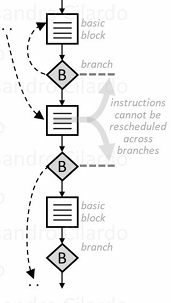
\includegraphics[width=0.28\textwidth]{fig/chapter_2/control_dependencies.png}}
\end{figure}


\noindent La predizione del branch a cui saltare però nella pratica non è mai perfetta, e avviene tramite meccanismi hardware (quelli di base sono descritti nel paragrafo [\ref{subsec:control_hazards}]) e software, come l'inserimento di un bit di indizio staticamente inserito nell'istruzione. Osserviamo che poichè il branch predictor \textit{scommette} sulla prossima istruzione da caricare, non fermando mai la pipeline, sono necessari meccanismi di \textbf{commit} o \textbf{rollback} per non comporomettere in maniera irreversibile lo stato del processore o peggio ancora della memoria. 

\subsection{Generalizzazione predittore a 2 bit}
Un predittore dinamico (hardware) a due bit è posizione a monte della fase issue. Il suo scopo è associare ad ogni istruzione di salto una predizione, ovvero un indirizzo target. Questo avviene consultando una memoria associativa, la cui chiave è un sottoinsieme dei bit dell'istruzione di salto. 

\begin{warn}
    di solito per indicizzare la branch history table si usano i bit meno significativi dell'istruzione di salto. Questo perchè si vuole mantenere contenuta la dimensione spaziale della tabella senza implementare meccanismi di decodifica o di hashing. Ciò significa eventualmente accettare collisioni, ma questo è un problema solo di performance, risolvibile e tollerabile se sufficientemente raro. Infatti i cambiamenti allo stato della memoria e del processore diventano effettivi solo quando la condizione del salto viene calcolata in fasi più avanzate della pipeline.
\end{warn}

I predittori a due livelli introducono un inerzia nel cambio di decisione per massimizzare l'efficienza nel caso di due loop innestati. Questa tecnica può essere generalizzata. Infatti è possibile costruire predittori a n bit, rendendo disponibili $2^n$ stati per la decisione e potendo arbitrariamente scegliere una tra le transizioni di stato che generano il cambio di decisione.  

\begin{figure}[ht]
    \centering
    \setlength{\fboxrule}{0.5pt} % spessore sottile
    \setlength{\fboxsep}{0pt}    % senza spazio interno
    \fbox{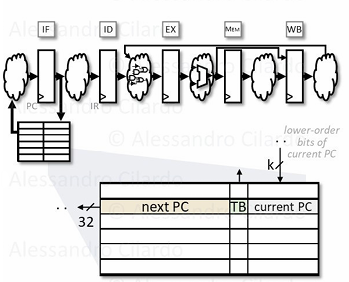
\includegraphics[width=0.45\textwidth]{fig/chapter_2/n_bit_predictor.png}}
\end{figure}


\noindent Succede spesso che l comportamento di un branch sia correlato a quello di diversi altri branch presenti nel codice. L'informazione sull'esito dei branch correlati può essere utile nel determinare la predizione. Si può pensare quindi di rendere la predizione locale dipendente dalla storia \textit{globale} dei salti, ovvero dal comportamento degli ultimi m salti, indipendentemente da dove si trovavano nel codice (per questo globale). \uppercase{è} naturale quindi implementare questa \textit{storia} come uno shift register a m bit.  
Così si costruiscono meccanismi hardware, denominati (m,n)-predittori, che in base al comportamento globale scelgono una delle $2^m$ branch history tables da consultare. Questo meccanismo è veloce ed efficace, ma richiede diverse iterazioni per andare a regime. Quindi è ragionevole usarlo in caso di molte iterazioni che coinvolgono diversi salti. Osserviamo che questo meccanismo approssima una tecnica di machine learning di \textit{addestramento} per una predizione. 

\begin{warn}
    Il numero di branch history tables da consultare cresce esponenzialmente con m, quindi bisogna cercare un trade off tra efficienza e consumo di risorse.  
\end{warn}

\begin{figure}[ht]
    \centering
    \setlength{\fboxrule}{0.5pt} % spessore sottile
    \setlength{\fboxsep}{0pt}    % senza spazio interno
    \fbox{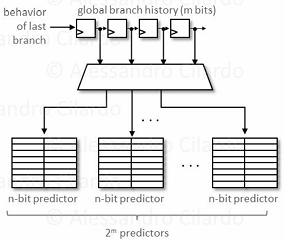
\includegraphics[width=0.45\textwidth]{fig/chapter_2/predittore_m_n.png}}
\end{figure}

\noindent Alcune tecnologie mirano all'implementazione di un predittore di indirizzo, oltre che ad un predittore di esito del salto. Questo è utile in casi come istruzioni di ritorno da subroutine, in cui il campo \textit{next PC} non è noto staticamente, ma deve essere recuperato nello stack. In alcuni processori moderni viene contemplata l'esistenza di una stack utilizzata soltanto per contenere indirizzi di ritorno, in modo da semplificare e velocizzare il recupero (questa memoria è alla base di molti attacchi di tipo \textit{code injection}). 

\begin{info}
    i problemi di indirizzo determinato dinamicamente possono essere risolti staticamente da software, attraverso le espansioni \textit{inline} delle funzioni, in modo da determinare a tempo di compilazione (sfruttando meccanismi di memoria virtuale) l'indirizzo a cui saltare.  
\end{info}

\subsection{Gestione delle eccezioni}
Nel modello di esecuzione out of order, le eccezioni possono occorrere in uno stage qualsiasi della pipeline. Per un richiamo su come vengono gestite le eccezioni in una pipeline semplice a cinque stadi, consultare il paragrafo [\ref{subsec:control_hazards}].

\noindent Per quanto riguarda l'approccio speculativo, è possibile permettere alle istruzioni di procedere fino alla fase di WB, anche quando non è sicuro che debbano essere eseguite. Chiaramente serve un meccanismo di ripristino qualora la speculazione fosse sbagliata. La speculazione hardware ha quindi bisogno di una fase \textit{commit} aggiuntiva. 
Il workflow diventa \textbf{issue} (in order) $\rightarrow$ \textbf{OpRead, EXE, WB} (out of order) $\rightarrow$ \textbf{commit} (in order).
Le istruzioni possono leggere risultati ancora non commitati da istruzioni precedenti, attraverso un buffer temporaneo, non direttamente dai registri. 

\noindent Una particolare tecnica utilizzata per la speculazione hardware è il \textbf{Re-Order Buffer} (ROB). Questo buffer traccia le istruzioni complete ma non committate e mantiene gli operandi di queste istruzioni tra il completamento e il commit. Usato in combinazione con lo schema di Tomasulo, i dati sono bufferizzati anche all'interno delle Reservation stations tra la fase di issue ed execute. 

\begin{figure}[ht]
    \centering
    \setlength{\fboxrule}{0.5pt} % spessore sottile
    \setlength{\fboxsep}{0pt}    % senza spazio interno
    \fbox{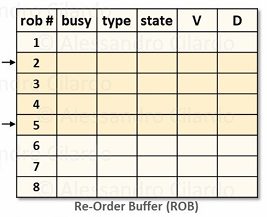
\includegraphics[width=0.4\textwidth]{fig/chapter_2/ROB.png}}
\end{figure}

\noindent ROB è gestito come una coda circolare, con puntatori per gestire la testa e la coda. I campi del ROB hanno il seguente significato:

\begin{description}[style=nextline,leftmargin=3.45cm,labelwidth=2.8cm,labelsep=0.4cm,font=\ttfamily\bfseries, itemsep=0.01em]
\item[rob \#] Identifica le operazioni 
\item[type] usato per distinguere le operazioni di store e tracciare i salti 
\item[state] Flag che indica se il campo V è valido 
\item[D] Registro target in scrittura 
\item[V] Valore da scrivere nel registro   
\end{description}

\noindent Le Reservation Station subiscono delle modifiche, in particolare i campi $S_i$ vengono sostituiti dalle entry $rob_i$, mentre il campo D viene sostituito da $D_rob$. Analogamente la status register table conterrà due campi per ogni registro (busy, rob) in cui viene indicato se una particolare operazione aspetta di effettuare il commit di una scrittura su quel particolare registro.  
Il funzionamento dello schema di Tomasulo con ROB è il seguente: Le istruzioni vengono recuperate in ordine, e seguono gli steps Issue, Execute, WriteBack e Commit. Un'istruzione vienne accettata se è disponivile un appropriato slot delle Reservation Staions ed è disponibile una ROB entry. Una volta accettata, l'operazione viene inserita nella ROB e viene aggiornata la RS e la Register Status Table. L'esecuzione avviene appena tutti i dati sono disponibili e copiati nei campi $V_i$. Nella fase WriteBack, attraverso il common data bus il ROB Value viene trasmesso in broadcast, in modo che le RS possano eventualmente accettarlo. Infine, la fase di commit esamina la coda ROB in testa, e se è il caso di predizione errata si effettua il flush della tabella fino alla coda. Altrimenti, si procede con il commit e si fa avanzare il puntatore coda. Osserviamo che sono ancora possibili hazards strutturali, ma costruire RSs e ROB più larghi è meno costoso che implementare più unità funzionali. 

\begin{figure}[ht]
    \centering
    \setlength{\fboxrule}{0.5pt} % spessore sottile
    \setlength{\fboxsep}{0pt}    % senza spazio interno
    \fbox{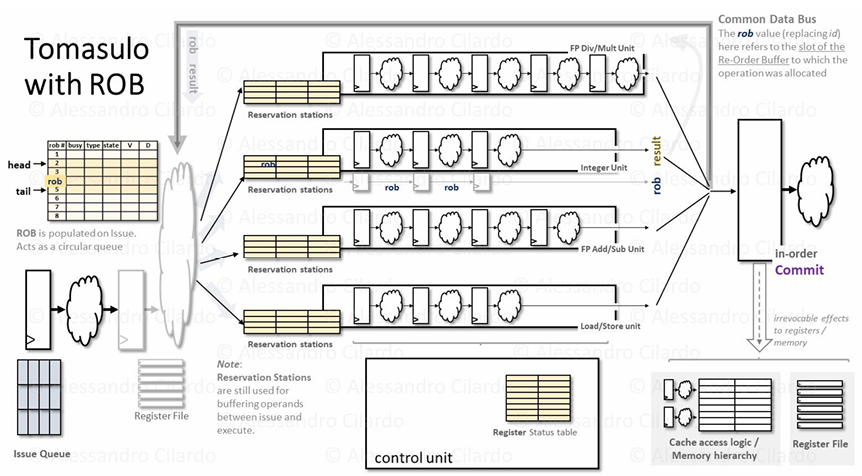
\includegraphics[width=0.75\textwidth]{fig/chapter_2/tomasulo_rob.png}}
\end{figure}

\noindent Grazie a questo schema è possibile committare e quindi scrivere più istruzioni per colpo di clock, superando uno dei bottleneck della pipe. Si può pensare di superare anche il bottleneck dovuto al fatto che la pipeline esegue una sola issue alla volta.
